\documentclass[12pt, notitlepage, final]{article}

\newcommand{\name}{Vince Coghlan and Zack Vogel}

%\usepackage[dvips]{graphics,color}
\usepackage{amsfonts}
\usepackage{amssymb}
\usepackage{amsmath}
\usepackage{latexsym}
\usepackage{enumerate}
\usepackage{amsthm}
\usepackage{nccmath}
\usepackage{setspace}
\usepackage[pdftex]{graphicx}
\usepackage{epstopdf}
\usepackage[siunitx]{circuitikz}
\usepackage{tikz}
\usepackage{float}
\usepackage{cancel}
\usepackage{setspace}
\usepackage{overpic}
\usepackage{mathtools}
\usepackage{listings}
\usepackage{color}
\usepackage{qtree}
%\usepackage{gensymb}

\usetikzlibrary{calc}
\usetikzlibrary{matrix}
\usetikzlibrary{positioning}

%\numberwithin{equation}{section}
\newcommand{\dbr}[1]{d_{\mbox{#1BR}}}
\newtheorem{lemma}{Lemma}
\newtheorem*{corollary}{Corollary}
\newtheorem{theorem}{Theorem}
\newtheorem{proposition}{Proposition}
\theoremstyle{definition}
\newtheorem{define}{Definition}

\newdimen\digitwidth{}
\settowidth\digitwidth{0}
\def~{\hspace{\digitwidth}}

\setlength{\parskip}{1pc}
\setlength{\parindent}{0pt}
\setlength{\topmargin}{-3pc}
\setlength{\textheight}{9.0in}
\setlength{\oddsidemargin}{0pc}
\setlength{\evensidemargin}{0pc}
\setlength{\textwidth}{6.5in}

\DeclareMathOperator*{\argmin}{arg\,min}

%absolute value code
\DeclarePairedDelimiter\abs{\lvert}{\rvert}%
\DeclarePairedDelimiter\norm{\lVert}{\rVert}
\makeatletter
\let\oldabs\abs{}
\def\abs{\@ifstar{\oldabs}{\oldabs*}}
%
\let\oldnorm\norm{}
\def\norm{\@ifstar{\oldnorm}{\oldnorm*}}
\makeatother

\def\dbar{{\mathchar'26\mkern-12mu d}}
%\def \P[x]{\Frac{\partial}{\partial x}}
%\def \D[x]{\Frac{d}{dx}}
\newcommand{\PD}[2]{\frac{\partial#1}{\partial#2}}
\newcommand{\PF}[1]{\frac{\partial}{\partial#1}}
\newcommand{\DD}[2]{\frac{d#1}{d#2}}
\newcommand{\DF}[1]{\frac{d}{d#1}}
\newcommand{\fix}[2]{\left(#1\right)_#2}
\newcommand{\ket}[1]{|#1\rangle}
\newcommand{\bra}[1]{\langle#1|}
\newcommand{\braket}[2]{\langle{} #1 | #2 \rangle}
\newcommand{\bopk}[3]{\langle{} #1 | #2 | #3 \rangle}
\newcommand{\Choose}[2]{\displaystyle{} {#1 \choose{} #2}}
\newcommand{\proj}[1]{\ket{#1}\bra{#1}}
\def\del{\vec{\nabla}}
\newcommand{\avg}[1]{\langle#1\rangle}
\newcommand{\piecewise}[4]{\left\{\beginProtected{array}{rl}#1&:#2\\#3&:#4\endProtected{array}\right.}
\newcommand{\systeme}[2]{\left\{\beginProtected{array}{rl}#1\\#2\endProtected{array}\right.}
\def\Godel{G$\ddot{\mbox{o}}$del}

\title{Analog Android Drum Machine}
\date{\today}
\author{\name\\ECEN3000}

\begin{document}

\maketitle

\section{Introduction}
Analog drum machines are used by many modern musicians as a matter of convinience, and that is indeed why
they were initially created.  After many years of musical development, however, the sounds of a real
analog drum machine are now associated with artists like Kanye West, Todd Terje, Can, and Marvin Gaye.  With
modern technology, any normal person can take a great photograph, or make a good movie.  Smartphones and
miniature CCD technology have allowed for the typical consumer to become an artist, expressing their creativity
with very little talent.  This is, however, not the case with music.  One needs to spend months learning the guitar,
playing drums, annoying the neighbors, and hurting fingers to create anything that is even somewhat pleasant.
With a drum machine, a regular person can become an artist.  With a few button clicks, it will do exactly what
you want with perfect tempo.  Modern drum machines like the famous TR-808~\cite{tr808} and Oberheim DMX~\cite{dmx}
cost upwards of \$1000. This is due to the high quality components, the difficulty of design and manufacture, and
the vast array of features.  We wanted to make a drum machine that could be used from a cell phone, and that only
costs a few dollars.

\section{Background}
An analog drum machine is a seemingly complicated set of circuits that, through the magic of electronics, is suprisingly
simple.  A drum sound is really just a decaying sine wave at a specific frequency.  For a bass drum that frequency might
be 20--50Hz, for a high tomb, that might be 150+Hz.  To achieve this, a short pulse is sent into an op-amp, which then
oscilates as it slowly decays.  This sounds quite realistic, but it doesnt have to.  We want to achieve the clasic analog
drum sound, not a real drum design.  The oscilator circuit for the bass drum looks like so:
\begin{center}
\begin{circuitikz} \draw{}
  (4,4) node[op amp] (opamp) {}
  (opamp.+) node[left] {In}
  (opamp.-) to [short] (2,4.5)
    to [short] (2,9.4)
    to [R=$R_2$] (6,9.4)
    to [short] (6,4)
    to [short] (opamp.out)
  (2,8) to [C=$C_1$] (4,8)
    to [C=$C_2$] (6, 8)
  (4,8) to [R=$R_1$] (4,6.2)
    node[ground]{}
  (opamp.up) ++ (0,0.5) node[above] {$V_+$}
    -- (opamp.up)
  (opamp.down) ++ (0,-0.5) node[below] {$V_-$}
    -- (opamp.down)
  (6,4) to [short, -o] (7,4) node[right] {Out}
;\end{circuitikz}
\end{center}

This circuit, when given a pulse, will respond like so:
\begin{figure}[H]
\begin{center}
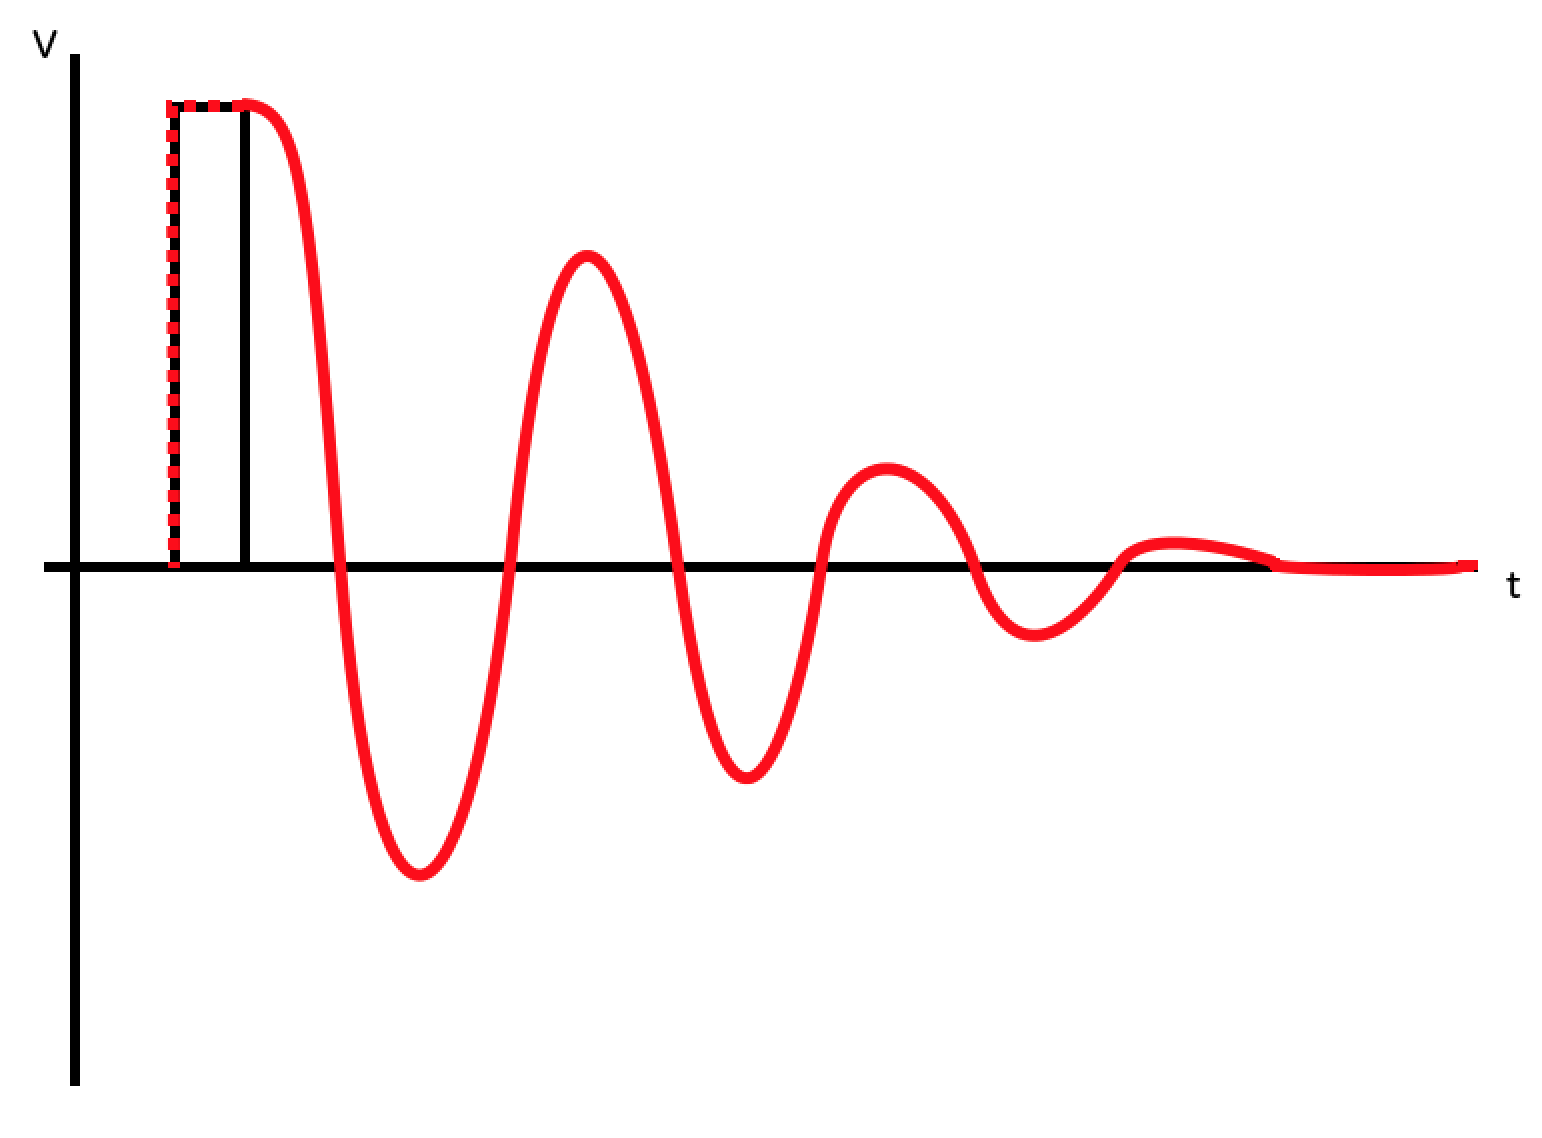
\includegraphics[width=8cm]{f1}
\end{center}
\end{figure}

Some circuit analysis will tell us that the frequency and quality is
\[
  f = \frac{1}{2\pi\sqrt{R_1R_2C_1C_2}} \text{  } Q = \frac{\sqrt{\frac{R_2}{R_1}}}{\sqrt{\frac{C_1}{C_2}}+\sqrt{\frac{C_2}{C_1}}}
\]
These equations and the circuit are given in~\cite{tr808}.  Changing any of these values will effect the frequency response
and the decay of the circuit.  These values aer quite difficult to get just right, the TR-808 implements $R_2$ as a large
potentiometer so that you can change the tune of the drum.  A snare drum is a combination of two sounds.  The sound of the drum,
and the sound of the snare.  This can be accomplished quite well by triggering the same drum circuit as above with a
decaying pulse of white noise.  The circuit for the white noise was also given in the schematics for the TR-808~\cite{tr808}:

\begin{figure}[H]
\begin{center}
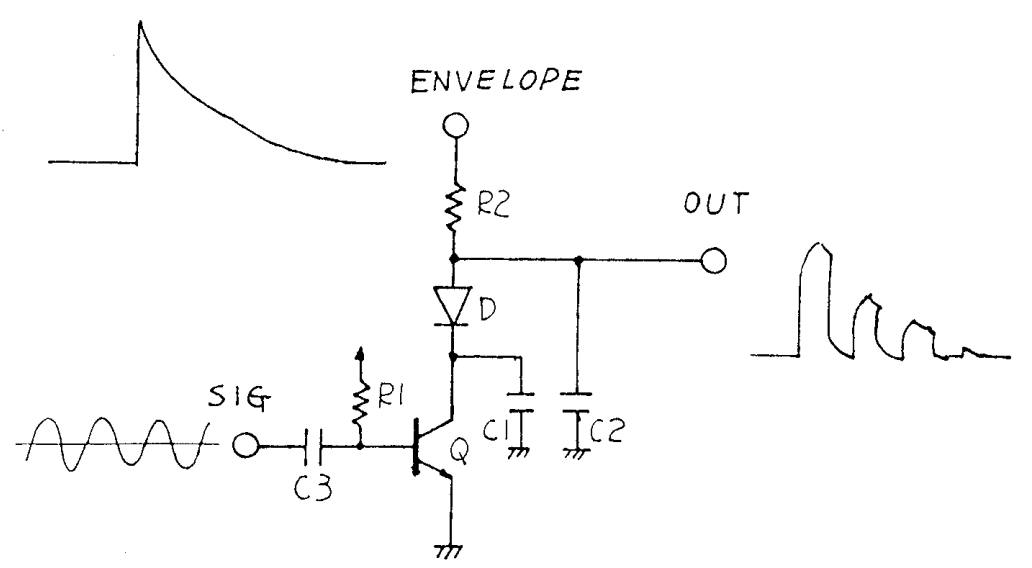
\includegraphics[width=12cm]{f2}
\end{center}
\end{figure}

The white noise was generated by a Linear Feedback Shift Register~\cite{lfsr}.  Additionally, our cymbal circuit is just
a decaying burst of the white noise.

All of these various instruments are then mixed in an op-amp and outputted in a two line interface to be fed into an
amplifier.

\newpage
\begin{thebibliography}{9}

  \bibitem{tr808}
  Roland Corporation,
  ``TR-808 Service Manual'',
  http://ericarcher.net/wp-content/uploads/2009/11/808-svc-man.pdf,
  1983.

  \bibitem{dmx}
  Oberheim Electronics,
  ``Obeheim DMX Schematics''
  http://www.electrongate.com/obfiles/index.html,
  1981.

\bibitem{lfsr}
  C. Stroud,
  ``Linear Feedback Shift Registers'',
  Dept. of ECE, Auburn,
  http://www.eng.auburn.edu/~strouce/class/elec6250/LFSRs.pdf,
  2004

\end{thebibliography}

\end{document}
